\documentclass[a4paper]{article}

\usepackage[brazil]{babel}
\usepackage{lipsum}
\usepackage{indentfirst}
\usepackage{graphicx}

\title{Projeto Final Lia (Nome Provisório)}

\author{Jonathas dos Santos \and Lucas Vinícius de Lima}

\begin{document}
    \maketitle
    
    \section{Descrição}
        % Lucas
        Nosso projeto é uma \emph{simulação} que se utiliza da tecnologia de
        \emph{Processamento de Linguagem Natural} (NPL) com a finalidade de
        auxiliar no aprendizado de uma língua estrangeira. Nosso programa
        simula, por meio do Pygame\footnote{Pygame é uma biblioteca python,
        voltada para a criação de jogos, construída sobre SDL trazendo
        funcionalidades e suporte a gráficos, manipulação de imagens, áudio,
        leitura de teclado e mouse, entre outros.}, uma barraquinha de feira com
        dois vendedores estrangeiros, que contém dos mais diversos produtos a
        venda, desde frutas a eletrônicos. O usuário sabe que os vendedores não
        conhecem sua língua, e como o educado cliente que é, interage com eles
        em sua língua natal. 

    \subsection{Funcionamento da simulação}

        Sobre a simulação, para iniciá-la, o usuário deve, por meio da fala, dar
        boas vindas aos vendedores no idioma que eles conhecem. Em seguida,
        pode lhes perguntar quais produtos estão disponíveis, ou se algum
        produto em específico está disponível. Pode fazer perguntas referente ao
        preço de certo produto, quantos produtos estão em estoque, ou até mesmo
        se há alguma encomenda especial. Quando o usuário decidir pagar por seus
        produtos, o vendedor lhe dirá em seu idioma, o valor da compra, e o
        usuário deverá entregar-lhe a quantidade correta. Após comprado o que
        desejava, o usuário, educado que é, dá uma despedida aos vendedores, e
        segue seu passeio na feira.

    \subsection{Escolha do cenário}

        A escolha do cenário de feira foi feita com o intuito de criar uma
        situação em que o usuário tenha contato com diversas palavras e
        expressões da língua. Na cena descrita, houve o contato com expressões
        para se iniciar uma conversa, para se despedir, o uso do modo
        interrogativo para saber quais produtos estão em estoque, o uso do modo
        afirmativo ou imperativo para se escolher quais produtos deseja, o
        contato com os diversos nomes de produtos, e o contato com números na
        hora do pagamento. 


    \section{Componentes do Projeto}
    \subsection{}
        Ao final, o projeto ficou subdividido em alguns módulos.
        
        \begin{table}[h]
            \center
            \begin{tabular}{|c|c|} \hline

            \end{tabular}
        \end{table}

    \section{Desenvolvimento do Projeto}
        
        A partir do momento em que estávamos com a proposta do projeto em mente,
        naturalmente nos dividimos em duas áreas de atuação: Lucas direcionou-se
        para o desenvolvimento \emph{`front-end'} e Jonathas direcionou-se para
        o desenvolvimento \emph{`back-end'}.

    \subsection{Front-end}

        O desenvolvimento do front-end engloba a criação da arte, e a
        programação no pygame.  A respeito da arte, fomos em busca de um
        artista e conseguimos a ajuda de \emph{João Pedro Ianke}. Ele foi
        o responsável por todos os desenhos, o que envolve tanto o cenário
        quanto os personagens e a UI.
        \marginpar{
            
\includegraphics[width=2.6cm]{jao.png}
            \small{\mbox{\textit{João Pedro Ianke}}}
        }

        \begin{figure}[!h]
            \center
            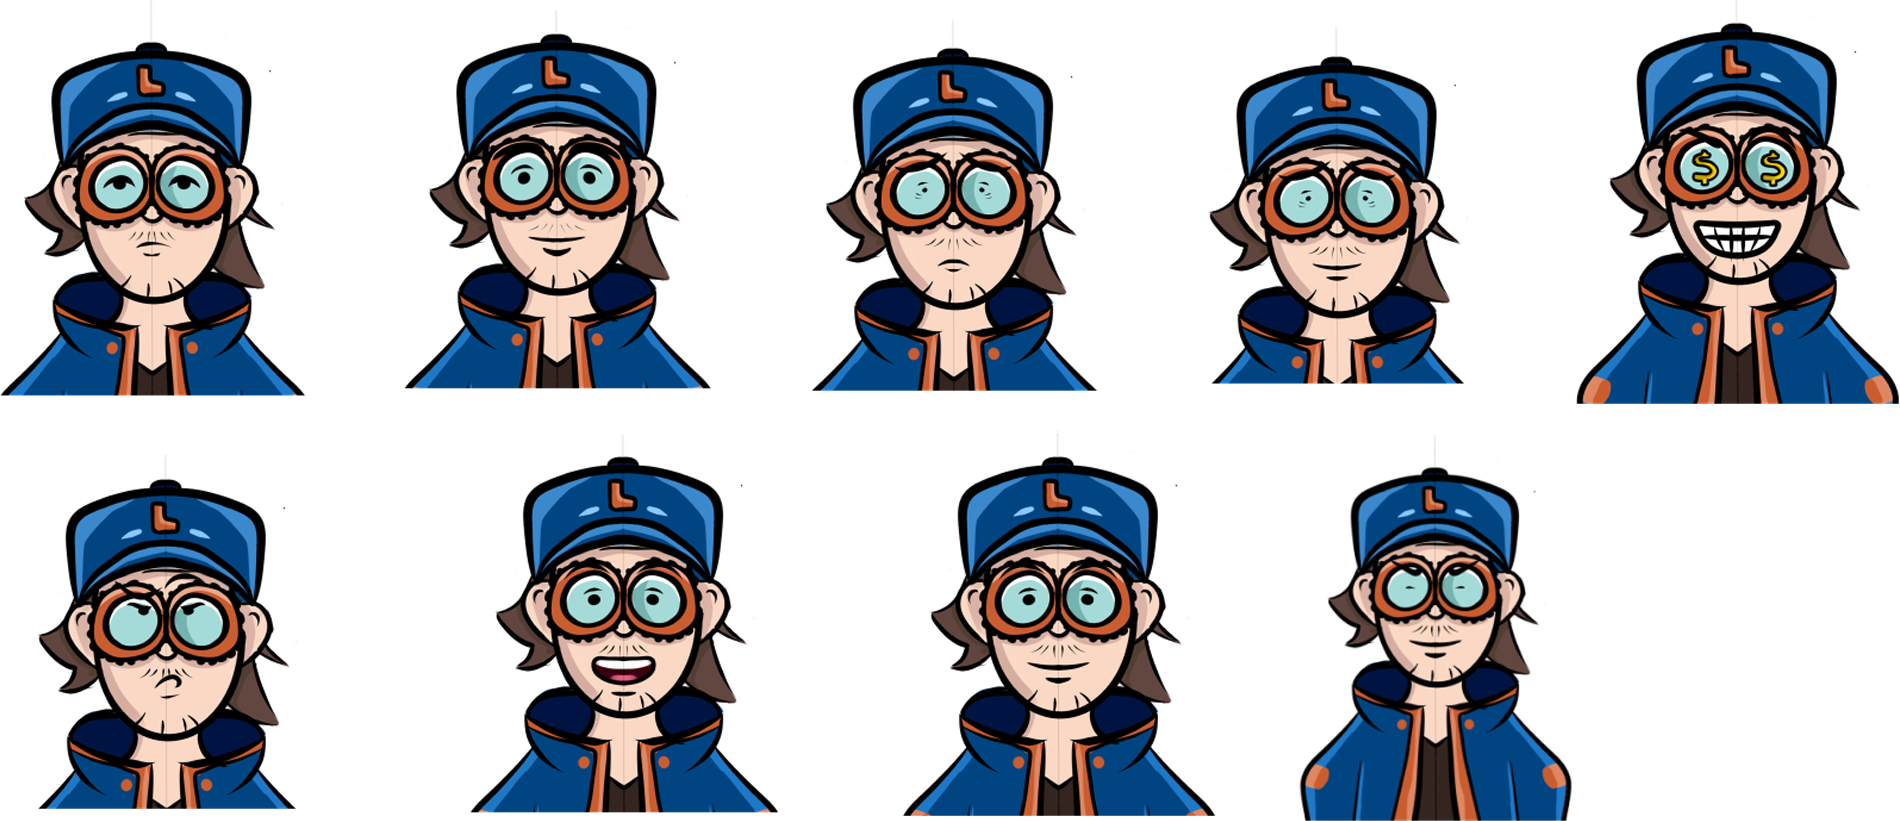
\includegraphics[width=8cm]{spreadsheet.png}
            \caption{Arte de conceito das expressões}
        \end{figure}
        
        O \emph{Pygame} foi a ferramenta para unir todos os elementos. Com os desenhos
        em mãos, fizemos a composição dos elementos na tela, 




        
    %\section{Passos Envolvidos}

    %\subsection{Preparação dos Dados}

    %\subsection{Construção do Modelo}

    %\subsection{Treinamento do Modelo}

    %\subsection{Ajuste fino do Modelo}

    %\subsection{Implantação do Modelo}

    %\section{Código do Projeto}


\end{document}
